\begin{sepframe}{History}
    {\scriptsize{Simplicity is the ultimate sophistication. L. Da Vinci}}
\end{sepframe}

\begin{frame}[fragile,c]
    \makebox[\linewidth]{\includegraphics[width=\paperwidth, height=\paperheight]{src/session/history/resources/diagram.pdf}}
\end{frame}

\begin{frame}
    \frametitle{History}
    \framesubtitle{Programming languages paradigms}

    \begin{itemize}[<+->]
        \item \textbf{O}bject \textbf{O}riented \textbf{P}rogramming
        \item \textbf{F}unctional \textbf{P}rogramming
        \item \textbf{I}mperative \textbf{P}rogramming
    \end{itemize}
\end{frame}

\begin{frame}[fragile,c]
    \frametitle{History}
    \framesubtitle{\textbf{I}mperative \textbf{P}rogramming}

    \makebox[\linewidth]{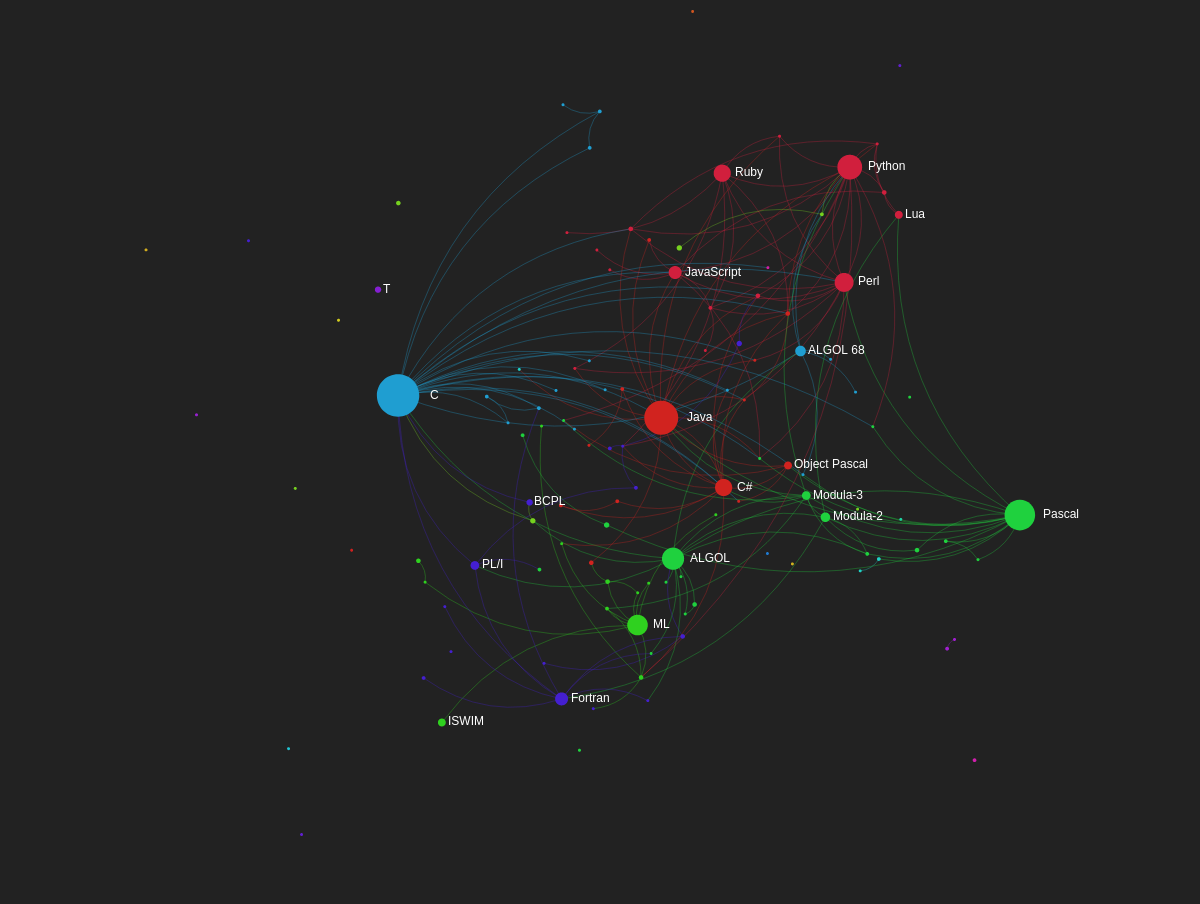
\includegraphics[width=\paperwidth, height=\paperheight]{src/session/history/resources/ip.png}}
\end{frame}

\begin{frame}[fragile,c]
    \lstinputlisting{src/session/history/resources/oop.js}
\end{frame}

\begin{frame}[fragile,c]
    \frametitle{History}
    \framesubtitle{\textbf{F}unctional \textbf{P}rogramming}

    \makebox[\linewidth]{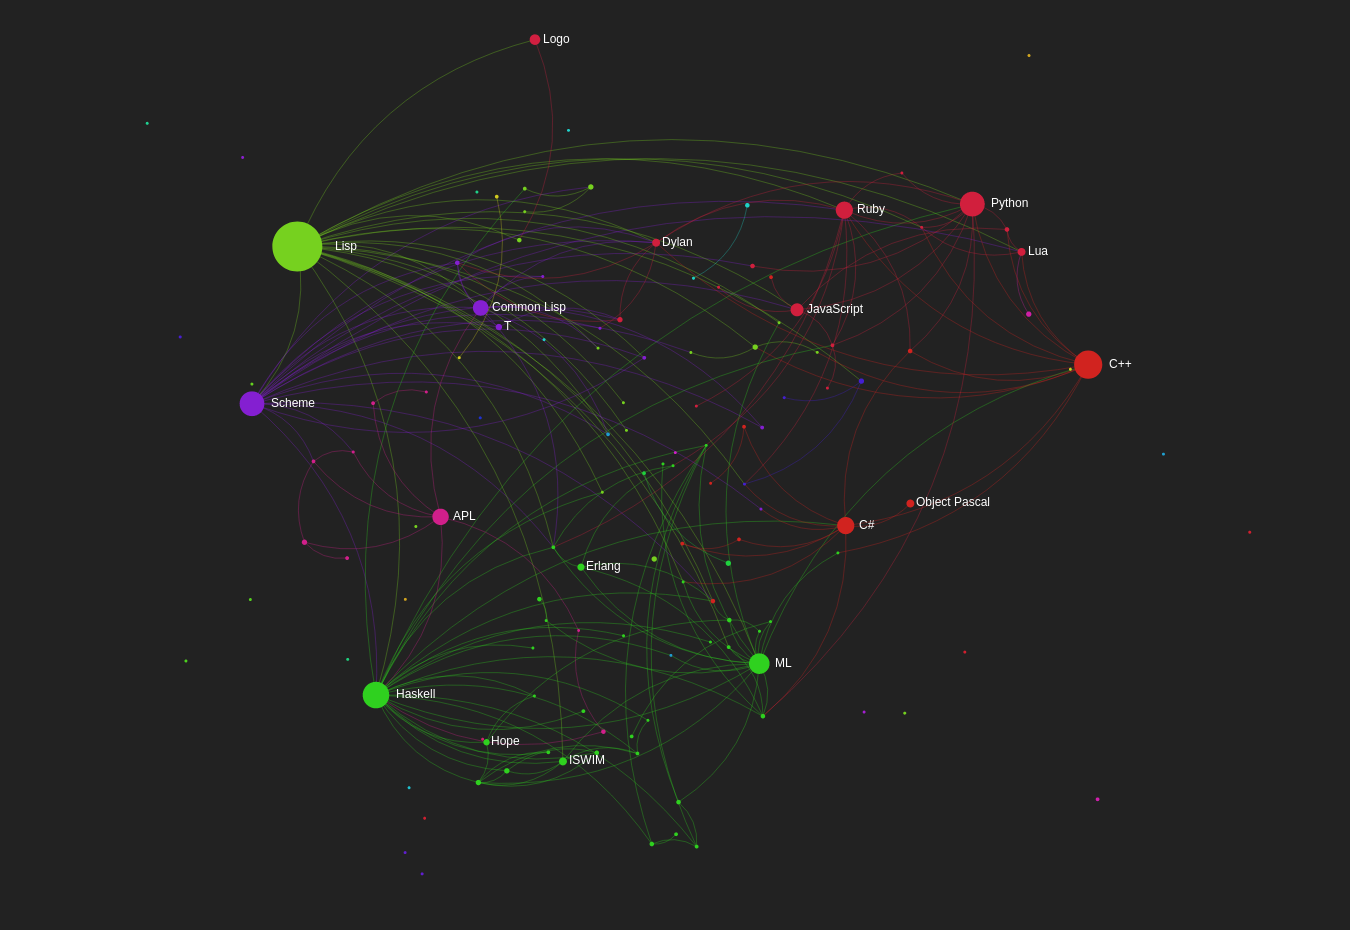
\includegraphics[width=\paperwidth, height=\paperheight]{src/session/history/resources/fp.png}}
\end{frame}

\begin{frame}[fragile,c]
    \lstinputlisting{src/session/history/resources/fp.js}
\end{frame}

\begin{frame}[fragile,c]
    \frametitle{History}
    \framesubtitle{\textbf{O}bject \textbf{O}riented \textbf{P}rogramming}

    \makebox[\linewidth]{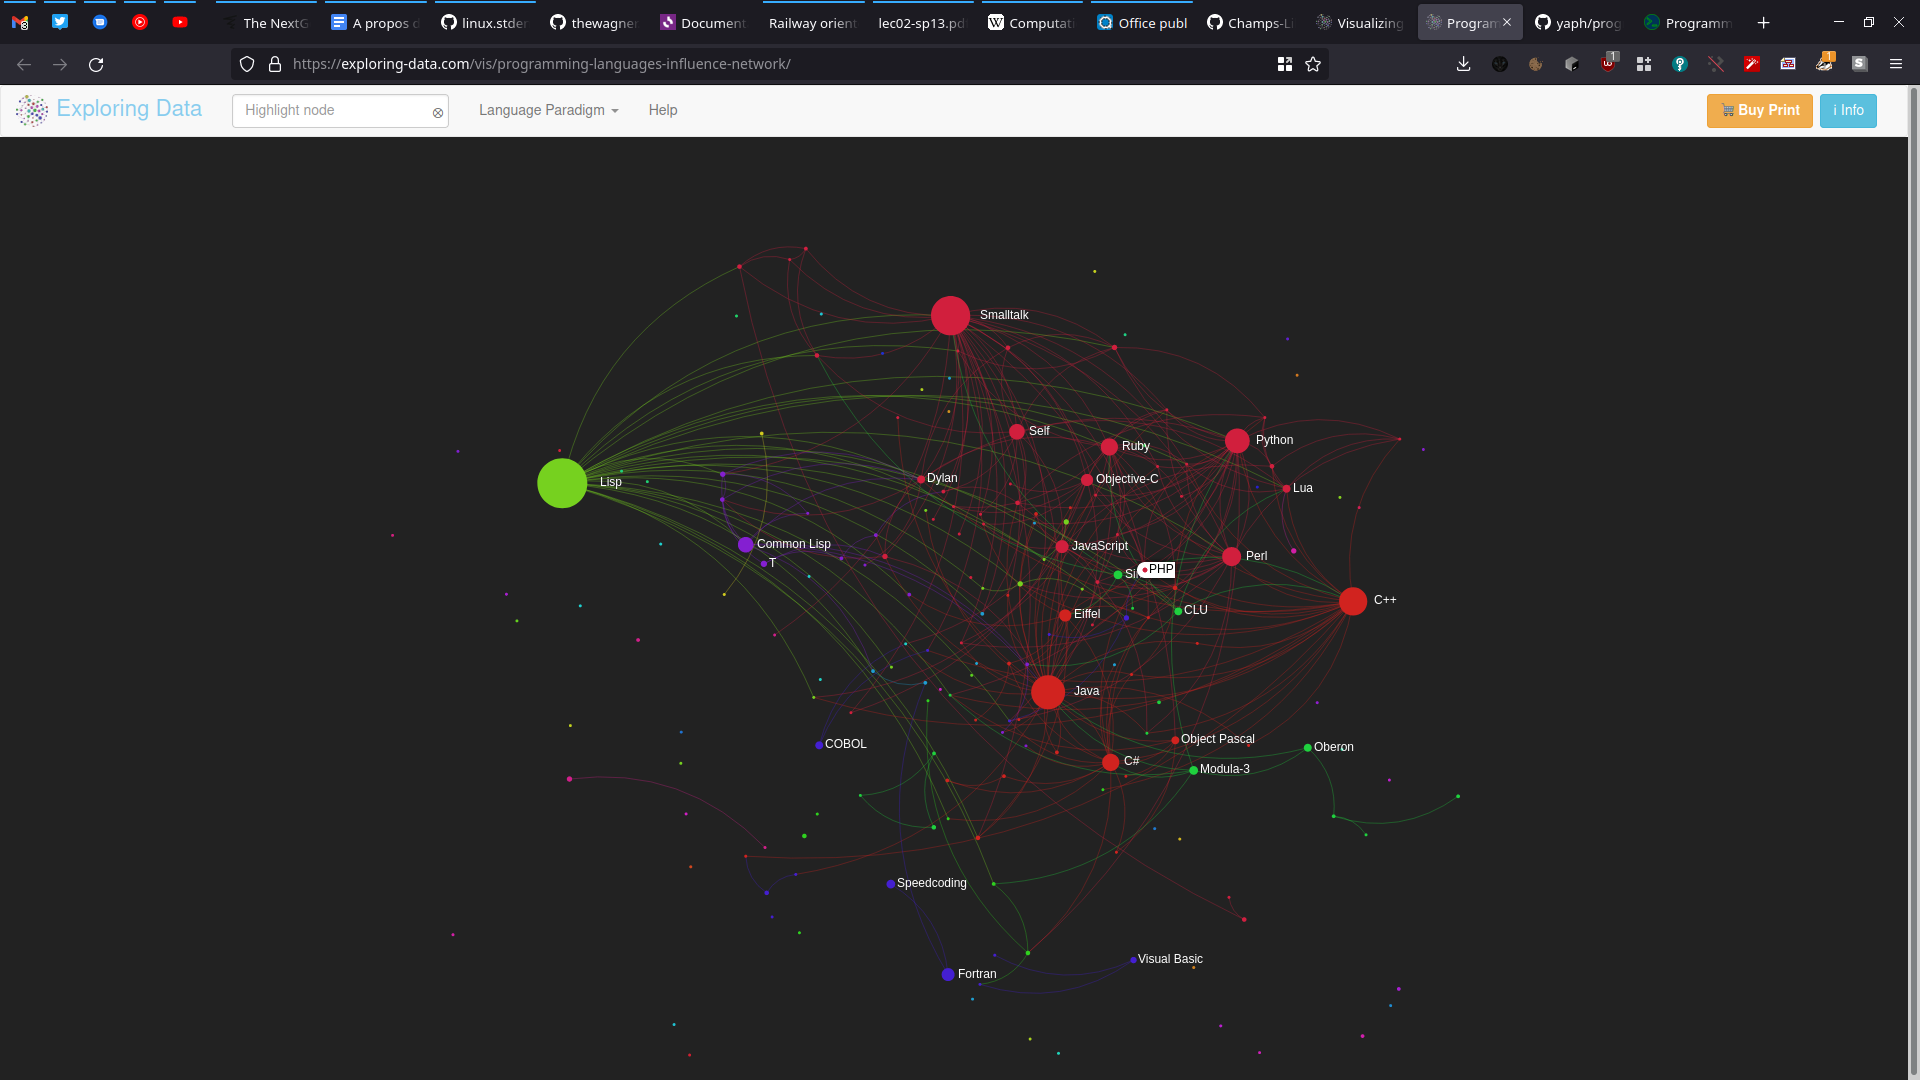
\includegraphics[width=\paperwidth, height=\paperheight]{src/session/history/resources/oop.png}}
\end{frame}

{
    \usebackgroundtemplate{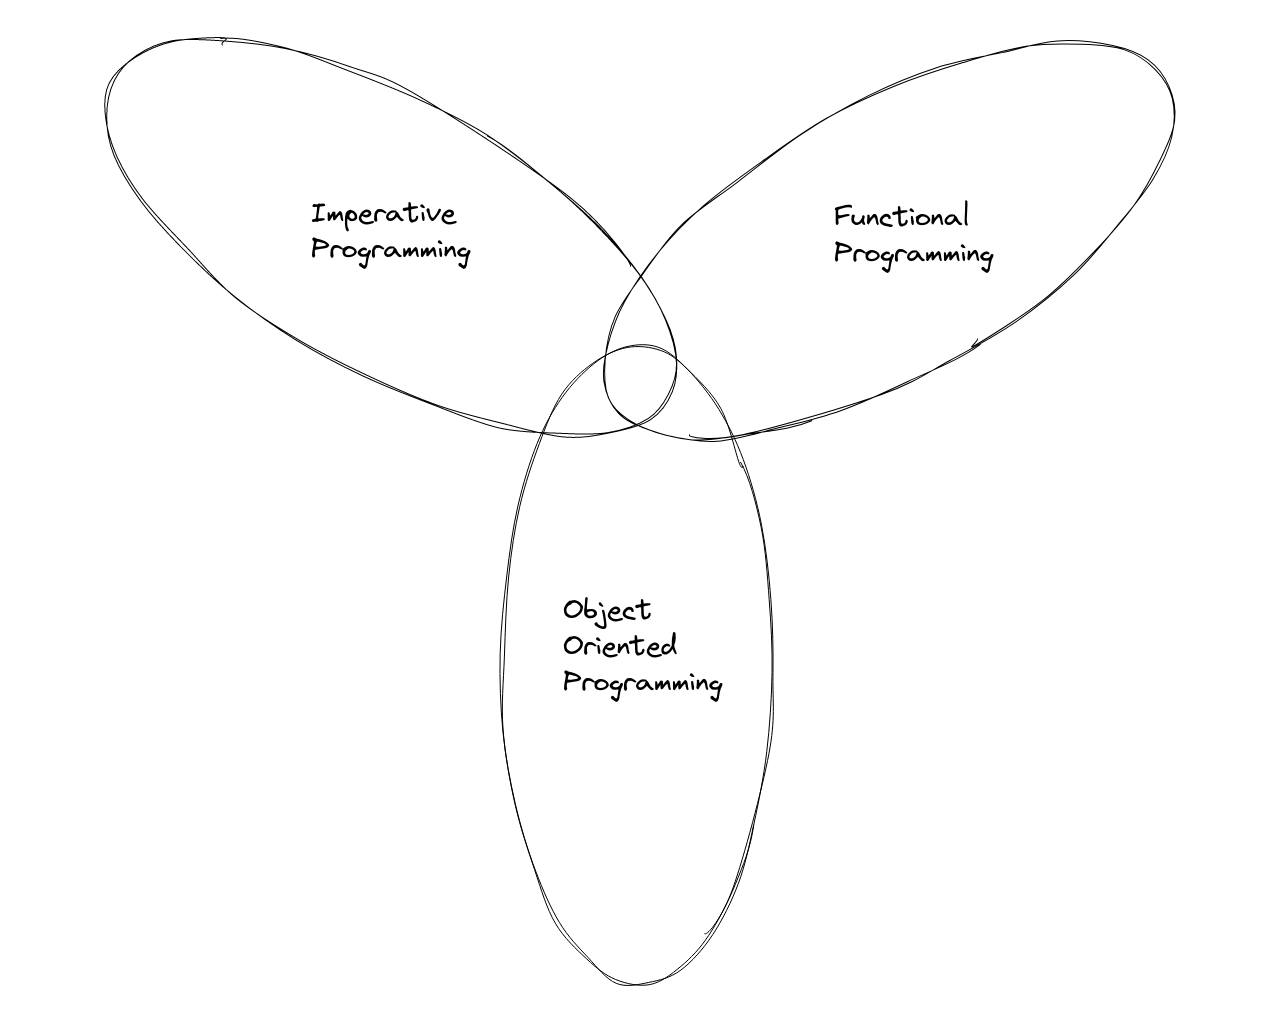
\includegraphics[keepaspectratio=true, width=\paperwidth, height=\paperheight]{src/session/history/resources/venn.png}}
    \setbeamertemplate{navigation symbols}{}
    \begin{frame}
    \end{frame}
}

\begin{frame}{My cool three points}
    \begin{itemize}
      \item<1-|alert@1> Point 1
      \item<3-|alert@3> Point 2
      \item<5-|alert@5> Point 3
    \end{itemize}
  \end{frame}
